
Dans ce chapitre nous nous int\'eressons \`a une classe tr\`es importante
de processus du second ordre, les processus autor\'egressifs \`a
moyenne ajust\'ee ou processus ARMA. Afin de pouvoir \'etudier
leurs propri\'et\'es, nous allons tout d'abord \'etablir les propri\'et\'es
des processus obtenus par un filtrage lin\'eaire de processus stationnaires au
second ordre.


\section{Filtrages lin\'eaires de processus au second ordre}


On s'int\'eresse dans ce paragraphe aux propri\'et\'es du processus
$(Y_t)$ obtenu comme image du processus $(X_t)$ par le filtre
lin\'eaire suivant :
\begin{equation}\label{eq:filtrage_1}
Y_t=\sum_{k\in\mathbb{Z}}\psi_k X_{t-k}\;,
\end{equation}
o\`u $(\psi_k)$ est une suite de nombres complexes.
Lorsqu'il n'y a qu'un nombre fini de $\psi_k$ non nuls,
la somme (\ref{eq:filtrage_1}) est bien d\'efinie. On dit dans ce cas-l\`a
que le filtre est \`a r\'eponse impusionnelle finie.
La question devient plus d\'elicate lorsque l'on consid\`ere des
filtres \`a r\'eponse impulsionnelle infinie c'est \`a dire lorsque
le nombre de $\psi_k$ non nuls est infini. En effet, $Y_t$ d\'efini par
(\ref{eq:filtrage_1}) est la limite dans un sens \`a pr\'eciser, d'une
suite de variables al\'eatoires. Le th\'eor\`eme \ref{theo:filtragepassl}
donne un sens pr\'ecis \`a cette limite.

% Pour les processus stationnaires au second ordre, on consid\`ere des filtrages
% lin\'eaires \`a valeurs dans l'espace engendr\'e par toutes les combinaisons
% lin\'eaires du processus, \'etendues \`a toutes leurs limites $L^2$.

% \begin{definition}
%   Soit $X=\{X_t, t\in \Zset\}$ un processus du second ordre. On note
%   $\cH^X_\infty$ la fermeture dans $L^2(\Omega)$ du sous-espace engendr\'e par
%   les v.a. $\{X_t,\,t\in \Zset\}$,
% $$
% \cH^X_\infty = \cspan{X_t,\,t\in \Zset}\;.
% $$
% \end{definition}
% Cet ensemble est alors le sous-espace de $L^2(\Omega)$ contenant toute v.a. $Y$
% pour lesquelles il existe une suite d'\'el\'ements $(Y_n)_{n\geq1}$ de
% $\lspan{X_t,\,t\in \Zset}$ (l'espace des combinaisons lin\'eaires finies form\'ees
% d'\'el\'ements de $\{X_t, t\in \Zset\}$) qui converge vers $Y$ au sens $L^2$ quand
% $n\to\infty$, \textit{i.e.}
% $$
% \lim_{n\to\infty}\esp{\left|Y-Y_n\right|^2}\to 0 \; .
% $$


% On introduit l'{\em op\'erateur de retard} qui facilitera l'\'ecriture
% des filtrages lin\'eaires \`a valeurs dans $\cH^X_\infty$.

% \begin{definition}[Op\'erateur de retard]
%   Soit $\{X_t,\,t\in\Zset\}$ d\'efini sur $(\Omega,\cF,\PP)$ un processus du
%   second ordre. On d\'efinit l'op\'erateur de retard $B$ (comme {\em backshift} en
%   anglais) comme l'op\'erateur de l'espace $\cH^X_\infty$ dans lui-m\^{e}me
%   d\'efini par $B(X_t)=X_{t-1}$. (l'extension \`a $\cH^X_\infty$ tout entier est
%   obtenu en compl\'etant par lin\'earit\'e et densit\'e.)
% \end{definition}


% On a le r\'esultat suivant dont la preuve \'el\'ementaire est omise.
% \begin{proposition}
%   Soit $X=\{X_t,\,t\in\Zset\}$ un processus du second ordre. Supposons que $X$
%   soit de moyenne constante, pour tout $t$,
%   $\esp[X_t]=\mu$. Alors $X$ est stationnaire au second ordre si et seulement
%   si $B$ est une isom\'etrie de $\cH^X_\infty$ dans lui-m\^{e}me.
% \end{proposition}

% On note $B^k = B \circ B^{k-1}$ pour $k \geq 1$ les compositions successives de
% l'op\'erateur $B$.  Pour $k<0$, $B^k$ est d\'efini comme l'op\'erateur inverse de
% $B^{-k}$.

% \begin{remark}
%   On remarque que l'op\'erateur $B$ est tr\`es li\'e \`a l'op\'erateur $S^{-1}$. Une
%   diff\'erence essentielle est qu'il op\`ere sur un espace de v.a. (l'espace
%   $\cH^X_\infty$) alors que $S^{-1}$ op\`ere sur un espace de trajectoires
%   (l'espace $E^\Zset$). Cette relation est formellement donn\'ee par l'\'egalit\'e des
%   2 v.a.  $B(\Pi_t\circ X)=\Pi_t\circ S^{-1}\circ X$.
% \end{remark}

% Cette remarque permet imm\'ediatement d'adapter le cas des filtres RIF de
% l'exemple~\ref{exple:rif} au contexte d\'ecrit ci-dessus.
% Notons $\phi(B)=\sum_k\phi_kB^k$, o\`u $(\phi_k)_{k\in\Zset}$ est une
% suite \`a support fini. Alors, pour tout $t\in\Zset$,
% $$
% Y_t=\phi(B)(X_t)= \sum_k\phi_k X_{t-k}
% $$
% est un \'el\'ement de $\cH^X_\infty$. Il est ais\'e de calculer la moyenne et la
% covariance du processus obtenu $Y=\{Y_t,\,t\in\Zset\}$ en utilisant les
% propri\'et\'es de lin\'earit\'e et de sesquilin\'earit\'e de la covariance. Le th\'eor\`eme
% suivant traite un cas un peu plus g\'en\'eral, qui montre que ces calculs passent
% ais\'ement \`a la limite dans le cas d'une somme infinie, pourvu que
% $\sum_k|\phi_k|<\infty$. Cette condition ne permet cependant pas la description
% la plus g\'en\'erale du filtrage lin\'eaire \`a valeurs dans $\cH^X_\infty$, comme nous
% le verrons au paragraphe~\ref{sec:filtr-des-proc-theo-generale}.

\begin{theorem}
 \label{theo:filtragepassl}
 Soit $(\psi_k)_{k\in\Zset}$ une suite absolument sommable, \ie\ $\sum_{k= -\infty}^\infty |\psi_k| < \infty$
et soit $(X_{t})$ un processus al\'eatoire tel que $\sup_{t \in \Zset} \PE {|X_{t}|} < \infty$.
Alors, pour tout $t \in \Zset$, la suite~:
\[
Y_{n,t} = \sum_{k=-n}^n \psi_k X_{t-k}
\]
converge presque s\^urement, quand $n$ tend vers l'infini, vers
une limite $Y_t$ que nous notons
$$
Y_{t} = \sum_{k=-\infty}^\infty \psi_s X_{t-s}\eqsp.
$$
De plus, la variable al\'eatoire $Y_t$ est int\'egrable, \ie\ $\PE{|Y_t|} < \infty$ et la suite $(Y_{n,t})_{n \geq 0}$
converge vers $Y_t$ dans  $L^1\espaceproba$, \textit{i.e.}
$$
\limn \PE{ |Y_{n,t} - Y_{t}|} = 0 \eqsp.
$$
Supposons que $\sup_{t \in \Zset} \PE{|X_t|^2} < \infty$ alors
$\PE{|Y_{t}|^2} < \infty$ et la suite $(Y_{n,t})_{n \geq 0}$ converge en moyenne quadratique vers la variable
al\'eatoire $Y_{t}$, \textit{i.e.}
$$
\limn \PE {|Y_{n,t} - Y_{t}|^2} = 0 \eqsp.
$$
\end{theorem}
\begin{proof}\smartqed
Notons pour tout $t \in \Zset$ et $n \in \Nset$, $U_{n,t} = \sum_{k=-n}^{n} |\psi_k| |X_{t-k}|$. La suite
$(U_{n,t})_{n \geq 0}$ est une suite de variables al\'eatoires int\'egrables. Puisque $\limn \uparrow U_{n,t} = \sum_{k\in\Zset}|\psi_k| |X_{t-k}|$, on en d\'eduit que (th\'eor\`eme de Beppo-Levi)
$$
\lim_{n \to \infty} \uparrow \PE{U_{n,t}} = \PE{\sum_{k\in\zset}|\psi_k| |X_{t-k}|}\;,
$$
o\`u $\lim_{n \to \infty} \uparrow$ signifie qu'il s'agit d'une limite croissante.
Comme
$$
\PE{U_{n,t}}\leq \sum_{k=-n}^{n} |\psi_k| \PE{|X_{t-k}|} \leq \sup_{t \in \Zset} \PE{|X_t|} \, \sum_{k\in\Zset} |\psi_s|
<\infty\eqsp,
$$
on en d\'eduit que
\[
\PE {\sum_{k\in\Zset} |\psi_k| |X_{t-k}| }< \infty \eqsp.
\]
Par cons\'equent, il existe un ensemble $\Omega_0 \in \cF$ tel que $\PP(\Omega_0) = 1$
et tel que, pour tout $\omega \in \Omega_0$,
\[
\sum_{k\in\Zset} |\psi_k| | X_{t-k}(\omega) | < \infty\; .
\]
Donc pour tout $\omega \in \Omega_0$,
$$
|Y_{n,t}(\omega)-Y_t(\omega)|\leq\sum_{|k|>n}|\psi_k||X_{t-k}(\omega)|\to 0\;,\;
\textrm{lorsque } n\to\infty\;.
$$
Ainsi, pour tout $\omega \in \Omega_0$, $Y_{n,t}(\omega)$ est convergente et converge vers
$Y_t(\omega)$, ce qui montre que $\limn Y_{n,t}= Y_t$ \ps\ . Le lemme de Fatou montre que
\[
\PE{|Y_t|}= \PE{\liminf_n |Y_{n,t}|} \leq \liminf_n \PE{Y_{n,t}} \leq \sup_t \PE{|X_t|} \sum_{j=-\infty}^\infty |\psi_j| < \infty \eqsp,
\]
et donc que $Y_t \in \lone\espaceproba$. Comme $|Y_{n,t} - Y_t| \leq \sum_{k \in \Zset} |\psi_k| |X_{t-k}|$,
le th\'eor\`eme de convergence domin\'ee montre que $\lim_n \PE{|Y_{n,t}-Y_t|} = 0$ et donc que la suite
$\{ Y_{n,t} \}$ converge vers $Y_t$ dans $\lone\espaceproba$.

Consid\'erons maintenant le cas o\`u $\sup_{t \in \Zset}
\PE{|X_{t}|^2} < \infty$. Remarquons tout d'abord que $\PE{
|X_{t}|} \leq (\PE {|X_{t}|^2})^{1/2}$ et donc que cette condition
implique que $\sup_{t \in \Zset} \PE {|X_{t}|} < \infty$. La
suite $(Y_{m,t})_{m\geq 0}$ est une suite de Cauchy dans
$L^2\espaceproba$. En effet, pour $p \geq q$,
nous avons en notant $\| X \|_2 = \left( \PE{|X|^2} \right)^{1/2}$
\begin{multline*}
\|Y_{p,t} - Y_{q,t} \|_2 = \left\| \sum_{|k|=q+1}^p \psi_k X_{t-k} \right\|_2
\leq \sup_t \|X_t\| \sum_{|k|=q+1}^p |\psi_k|  \underset{q,p \rightarrow \infty}{\longrightarrow} 0\;.
\end{multline*}
Comme $L^2\espaceproba$ est complet, la suite $(Y_{n,t})$ converge vers une variable $Y_t^\star$.
En utilisant le lemme de Fatou, nous avons
\[
\PE{|Y_t - Y_t^\star|^2} = \PE{\liminf_n |Y_{n,t} - Y_t^{\star}|^2} \leq \liminf_n \PE{|Y_{n,t}- Y_t^{\star}|^2}= 0 \eqsp,
\]
ce qui montre que les limites \ps\ $Y_t$ et $\ltwo\espaceproba$, $Y_t^\star$ co\"{i}ncident \ps\ .

\end{proof}


Le r\'esultat suivant \'etablit que le processus $(Y_t)$ obtenu par filtrage
lin\'eaire d'un processus stationnaire au second ordre $(X_t)$ via
l'\'equation (\ref{eq:filtrage_1}) est
lui-m\^{e}me stationnaire au second ordre, \`a condition que la
suite des $(\psi_k)$ soit absolument sommable
\textit{i.e.} $\sum_{k\in\mathbb{Z}}|\psi_k|<\infty$.

\begin{theorem}[Filtrage des processus stationnaires au second ordre]
 \label{theo:filtragepassl_stat}
 Soit $(\psi_k)$ une suite
telle que $\sum_{k= - \infty}^\infty |\psi_k| < \infty$ et soit
$(X_{t})$ un processus stationnaire au second ordre de moyenne
$\mu_X= \PE{X_{t}}$ et de fonction d'autocovariance $\gamma_X(h)=
\cov(X_{t+h},X_{t})$ alors le processus $Y_{t} =
\sum_{k=-\infty}^\infty \psi_k X_{t-k}$ est stationnaire au second
ordre de moyenne~:
\begin{equation}
\label{eq:moyennefiltre}
 \mu_Y = \mu_X \sum_{k=-\infty}^\infty \psi_k\; ,
\end{equation}
de fonction d'autocovariance~:
\begin{equation}
\label{eq:facfiltrage}
 \gamma_Y(h)= \sum_{j=-\infty}^\infty
    \sum_{k=-\infty}^\infty \psi_j \bar{\psi}_k \gamma_X(h+k-j)\; ,
\end{equation}
et de mesure spectrale~:
\begin{equation}
\label{eq:dspfiltrage}
  \nu_Y(\rmd\lambda) = |\psi(\rme^{-i\lambda})|^2 \nu_X(\rmd\lambda)\; ,
\end{equation}
o\`u $\psi(\rme^{-\rmi \lambda}) = \sum_{k\in \zset} \psi_k \rme^{-\rmi k \lambda}$.
%est
%la transform\'ee de Fourier \`a temps discret de la suite $\{ \psi_k \}_{k \in \Zset}$.
%Enfin l'intercovariance entre
%les processus $Y_{t}$ et $X_{t}$ a pour expression~:
%\begin{equation}
% \label{eq:intercovfiltrage}
% \gamma_{YX}(h)=\PE{(Y_{t+h}-\mu_Y)(X_{t}-\mu_X)}
% = \sum_{k=-\infty}^\infty \psi_k \gamma_X(h-k)
% \end{equation}
\end{theorem}
\begin{proof}\smartqed
D'apr\`es la continuit\'e du produit scalaire dans $L^2\espaceproba$, voir th\'eor\`eme \ref{theo:cont_prod_int}, on a
\begin{multline*}
\PE{\sum_{k\in\Zset}\psi_k X_{t-k}}=\PE{\lim_{n\to\infty}\sum_{k=-n}^n \psi_k X_{t-k}}
=\lim_{n\to\infty}\PE{\sum_{k=-n}^n \psi_k X_{t-k}}\\
=\mu_X \left(\lim_{n\to\infty}\sum_{k=-n}^n \psi_k \right)
=\mu_X \sum_{k\in\Zset} \psi_k\; .
\end{multline*}

Montrons \`a pr\'esent le r\'esultat sur la fonction d'auto-covariance.
D'apr\`es la continuit\'e du produit scalaire dans $L^2\espaceproba$, voir th\'eor\`eme \ref{theo:cont_prod_int}, on a
\begin{equation*}
\Cov{Y_t}{Y_{t+h}} =\lim_{n\to\infty}\sum_{k,j=-n}^n\psi_k \bar{\psi}_j\Cov{X_{t-k}}{X_{t+h-j}}
= \sum_{k\in\Zset}\psi_k \bar{\psi}_j\gamma_X(h+k-j)\; ,
\end{equation*}
ce qui montre Eq.~\eqref{eq:facfiltrage}
% Pour la fonction
% d'autocovariance, notons tout d'abord que, pour tout $n$, le
% processus $Y_{n,t} = \sum_{s=-n}^n \psi_s X_{t-s}$ est
% stationnaire au second ordre et que nous avons~
% \[
%  \cov(Y_{n,t},Y_{n,t+h})
%   = \sum_{j=-n}^n \sum_{k=-n}^n \psi_j \psi_k
%           \gamma_X(h+k-j)
% \]
% Remarquons ensuite que
% \begin{align*}
%  \cov( Y_{t},Y_{t+h})
%  &= \cov( Y_{n,t} + (Y_{t}-Y_{n,t}), Y_{n,t+h} + (Y_{t+h}-Y_{n,t+h})) \\
%  &= \cov( Y_{n,t}, Y_{n,t+h}) + \cov( Y_{t}- Y_{n,t},Y_{n,t+h}) \\
%     &+ \cov(Y_{n,t}, Y_{t+h}-Y_{n,t+h}) +
%     \cov(Y_{t}-Y_{n,t},Y_{t+h}-Y_{n,t+h})\\
%  &=A+B+C+D
% \end{align*}
% L'in\'egalit\'e~:
% \[
% \Var{Y_{n,t}-Y_{t}}
%    = \lim_{p \rightarrow \infty} \Var(Y_{n,t} - Y_{p,t})
%    \leq \left(\sum_{j=n+1}^\infty |\psi_j| \right)^2 \gamma_X(0)
% \]
% permet ensuite de d\'eduire, quand $n$ tend vers l'infini, les
% limites suivantes
% \begin{align*}
% &|B|
%   \leq (\Var{Y_{t}- Y_{n,t}})^{1/2} (\Var{Y_{n,t+h}} )^{1/2} \rightarrow 0 \\
% &|C|
%   \leq (\Var{Y_{t+h}- Y_{n,t+h}})^{1/2} (\Var{Y_{n,t}} )^{1/2} \rightarrow 0 \\
% &|D|
%   \leq (\Var{Y_{t+h}-Y_{n,t+h}})^{1/2} (\Var{Y_{t}- Y_{n,t}} )^{1/2} \rightarrow 0
% \end{align*}
% et donc $\cov( Y_{t},Y_{t+h}) = \limn\cov( Y_{n,t},Y_{n,t+h})$, ce
% qui d\'emontre l'expression~(\ref{eq:facfiltrage})
% ~\footnote{Nous
% venons ici de d\'emontrer directement la propri\'et\'e de continuit\'e de
% la covariance dans $L^2$ que nous verrons comme une cons\'equence de
% la structure d'espace de Hilbert au chapitre~\ref{chap:Prediction}.}.

D'apr\`es le th\'eor\`eme \ref{theo:herglotz},
$\gamma_X(h)=\int_\tore
\rme^{\rmi h \lambda}\nu_X(\rmd\lambda)$ o\`u $\nu_X$ d\'esigne la mesure
spectrale du processus $(X_{t})$.
En reportant cette expression de $\gamma_X(h)$ dans
\eqref{eq:facfiltrage}, nous obtenons
\begin{equation}\label{eq:gam_Y_spec}
 \gamma_Y(h)= \sum_{j=-\infty}^\infty \sum_{k=-\infty}^\infty
          \psi_j \bar{\psi}_k \int_\tore \rme^{\rmi (h+k-j)\lambda} \nu_X(\rmd\lambda)\;.
\end{equation}
Puisque
\[
\sum_{j=-\infty}^\infty \sum_{k=-\infty}^\infty
  \int_\tore |\psi_j| |\psi_k| \nu_X(\rmd\lambda)
  \leq \gamma_X(0) \left( \sum_{j=-\infty}^\infty |\psi_j| \right)^2<\infty\;,
\]
on peut appliquer le th\'eor\`eme de Fubini et permuter les
signes somme et int\'egrale dans \eqref{eq:gam_Y_spec}. Ce
qui donne~:
\[
\gamma_Y(h)
   = \int_\tore \rme^{\rmi h \lambda} \sum_{j=-\infty}^\infty \sum_{k=-\infty}^\infty
            \psi_j \bar{\psi}_k \rme^{\rmi k \lambda}\rme^{-\rmi j\lambda}
   = \int_\tore \rme^{\rmi h \lambda} |\psi(\rme^{-\rmi \lambda})|^2 \nu_X(\rmd\lambda)\;,
\]
o\`u $\psi(\rme^{-\rmi \lambda})=\sum_{k\in\Zset} \psi_k \rme^{-\rmi k \lambda}$.
On en d\'eduit, d'apr\`es le th\'eor\`eme \ref{theo:herglotz}
que $\nu_Y(\rmd\lambda) = |\psi(\rme^{-\rmi \lambda})|^2\nu_X(\rmd\lambda)$.
%  Pour d\'eterminer l'expression de
% l'intercovariance entre les processus entre les processus $Y_{t}$
% et $X_{t}$, il suffit de noter $|\cov(Y_{t+h},X_t)|^2 \leq
% \gamma_Y(0)\gamma_X(0)<+\infty$ et que~:
% \begin{align*}
%  \PE{(Y_{t+h}-\mu_Y)(X_t-\mu_X)}
%          &=\limn \cov (Y_{n,t+h},X_t)
%          =\limn \sum_{k=-n}^n \psi_k \cov(X_{t+h-k}X_t)\\
%          &=\sum_{k=-\infty}^{\infty} \psi_k \gamma_X(h-k)
% \end{align*}
% Ce qui conclut la preuve.

\end{proof}




% La relation~(\ref{eq:dspfiltrage}) qui donne la mesure spectrale
% du processus filtr\'e en fonction de la fonction de transfert du
% filtre et de la mesure spectrale du processus de d\'epart est
% particuli\`erement simple.
% \emnote{$\alpha(B)$ et $\beta(B)$ ne sont pas bien d\'efinis; je trouve que l'on devrait faire un \'enonc\'e de ce r\'esultat que l'on utilise dans la suite fr\'equemment}
% Elle montre par exemple que la mise
% en s\'erie de deux filtres $\alpha(B)$, $\beta(B)$ de r\'eponses
% impulsionnelles absolument sommables conduit \`aune mesure
% spectrale $|\alpha(\rme^{-\rmi\lambda})|^2 |\beta(\rme^{-\rmi\lambda})|^2
% \nu_X(\rmd\lambda)$ pour le processus filtr\'e, ce qui montre au
% passage que l'ordre d'application des filtres est indiff\'erent.

Nous d\'efinissons \`a pr\'esent une classe tr\`es importante de processus
obtenus par filtrage : les \emph{processus lin\'eaires} qui sont obtenus
en filtrant un bruit blanc.
\index{Processus!linaire}
\begin{definition}[Processus lin\'eaire]
\label{def:proc_lin}
Nous dirons que $(X_{t})$ est un \emph{processus lin\'eaire} s'il existe
un bruit blanc $Z_{t} \sim \BB(0,\sigma^2)$ et une suite de coefficients
$(\psi_k)_{k \in \Zset}$ absolument sommable telle que\,:
\begin{equation}
\label{eq:representationlineaire}
 X_{t}= \mu+\sum_{k=-\infty}^\infty \psi_k Z_{t-k},\quad t\in\zset\;,
\end{equation}
o\`u $\mu$ est un nombre complexe. On dira que $(X_t)_{t\in\zset}$ est un
processus lin\'eaire \emph{causal} par rapport \`a $(Z_t)_{t\in\zset}$
si~(\ref{eq:representationlineaire}) est v\'erifi\'ee avec $\psi_k=0$ pour tout
$k<0$.  On dira que $(X_t)_{t\in\zset}$ est un processus lin\'eaire
\emph{inversible} par rapport \`a $(Z_t)_{t\in\zset}$
si~(\ref{eq:representationlineaire}) est v\'erifi\'ee et qu'il existe de plus une
suite $(\pi_k)_{k\geq0}$ absolument sommable telle que
\begin{equation}
\label{eq:representationlineaireinversible}
 Z_{t}= \sum_{k=0}^\infty \pi_k \; (X_{t-k}-\mu),\quad t\in\Zset\;.
\end{equation}
\end{definition}
D'apr\`es le th\'eor\`eme \ref{theo:filtragepassl_stat}, un processus
lin\'eaire est stationnaire au second ordre de moyenne
$\mu$, de fonction d'autocovariance :
\begin{equation}\label{eq:gamm_proc_lin}
  \gamma_X(h)= \sigma^2 \sum_{j=-\infty}^\infty \psi_j \bar{\psi}_{j+h}= \sigma^2 \sum_{\ell=-\infty}^\infty \psi_{\ell-h} \bar{\psi}_{\ell}\eqsp,
\end{equation}
et dont la mesure spectrale admet une densit\'e  donn\'ee par :
\begin{equation}
  \label{eq:dps_modlin}
  f_X(\lambda) = \frac{\sigma^2}{2 \pi} |\psi(\rme^{-\rmi\lambda})|^2\; ,
\end{equation}
o\`u $\psi(\rme^{-\rmi\lambda}) = \sum_{k\in \zset} \psi_k \rme^{-\rmi k \lambda}$.
%==================================================
%==================================================
%==================================================



\section{Processus ARMA}
\label{s:procARMA}
%==================================================
% Dans ce paragraphe nous nous int\'eressons \`a une classe importante
% de processus du second ordre, les processus autor\'egressifs \`a
% moyenne ajust\'ee ou processus ARMA. Il s'agit de restreindre la
% classe des processus lin\'eaires en ne consid\'erant que les filtres
% dont la fonction de transfert est rationnelle.
%L'int\'er\^{e}t de cette param\'etrisation est qu'\`a partir d'un nombre fini de
%param\`etres, on peut approcher avec une pr\'ecision arbitraire toute densit\'e spectrale
%suffisamment r\'eguli\`ere.
%=====================================

Avant de passer au cas g\'en\'eral des processus ARMA, nous nous
int\'eressons \`a deux classes de processus ARMA particuliers :
les processus \`a moyenne ajust\'ee (MA) et les processus autor\'egressifs (AR).

\subsection{Processus MA$(q)$}
%=====================================
\begin{definition}[Processus MA($q$)]
On dit que le processus $(X_t)$ est \`a moyenne ajust\'ee d'ordre $q$ (ou MA($q$)) si $X_t$ est donn\'e par\,:
\begin{equation}
 \label{eq:recurrenceMAq}
 X_t= Z_t + \theta_1 Z_{t-1} + \cdots + \theta_q Z_{t-q}
\end{equation}
o\`u $Z_t \sim \BB(0,\sigma^2)$ et les $\theta_i$ sont des nombres complexes.
\end{definition}
Le terme ``moyenne ajust\'ee'' est la traduction assez malheureuse
du nom anglo-saxon ``moving average'' (moyenne mobile). Observons
que $X_t=\sum_{k=0}^q \theta_k Z_{t-k}$, avec la convention $\theta_0=1$.
En utilisant les r\'esultats du th\'eor\`eme~\ref{theo:filtragepassl_stat}, on obtient $\PE{X_t}=
0$, et
\begin{equation}
\label{eq:autocovariance-MA}
\gamma_X(h)=
\begin{cases}
\sigma^2 \sum_{t=0}^{q-h} \theta_k \bar{\theta}_{k+h}, & \text{si $0
  \leq h \leq q$}\;,\\
\sigma^2 \sum_{t=0}^{q+h} \bar{\theta}_k \theta_{k-h}, & \text{si $-q
  \leq h \leq 0$}\;,\\
 0, &\text{sinon}\;.
\end{cases}
\end{equation}
Enfin, d'apr\`es la formule~(\ref{eq:dps_modlin}), le processus
admet une densit\'e spectrale dont l'expression est :
$$
 f_X(\lambda)=\frac{\sigma^2}{2\pi}
     \left |1 + \sum_{k=1}^q \theta_k \rme^{-\rmi k\lambda} \right
     |^2\; .
$$
Un exemple de densit\'e spectrale pour le processus MA$(1)$ est
repr\'esent\'e sur la figure~\ref{fig:dspthMA1}.
%=====================================
\subsection{Processus AR$(p)$}
%=====================================
\begin{definition}[Processus AR($p$)]
On dit que le processus $\{ X_t \}$ est un processus autor\'egressif d'ordre $p$ (ou AR($p$)) si
$\{X_t \}$ est un processus stationnaire au second ordre et s'il est solution de l'\'equation de r\'ecurrence\,:
\begin{equation}
 \label{eq:recurrenceARp}
 X_t = \phi_1 X_{t-1} + \cdots + \phi_p X_{t-p} + Z_t\; ,
\end{equation}
o\`u $Z_t \sim \BB(0,\sigma^2)$ est un bruit blanc et les $\phi_k$ sont des nombres
complexes.
\end{definition}
Le terme ``autor\'egressif'' provient de la forme de l'\'equation~(\ref{eq:recurrenceARp}) dans
laquelle la valeur courante du processus s'exprime sous la forme
d'une r\'egression des
$p$ valeurs pr\'ec\'edentes du processus plus un bruit additif.

L'existence et l'unicit\'e d'une solution stationnaire au second ordre de
l'\'equation~(\ref{eq:recurrenceARp}) sont des questions d\'elicates (qui ne se posaient pas
lorsque nous avions d\'efini les mod\`eles MA). Nous d\'etaillons ci-dessous la r\'eponse \`a cette question
dans le cas $p=1$.

%======================================
\subsubsection{Cas~: $|\phi_1| < 1$}
%======================================
L'\'equation de r\'ecurrence (\ref{eq:recurrenceARp}) s'\'ecrit dans le cas $p=1$ :
\begin{equation}
\label{eq:recurrenceAR1}
        X_{t} = \phi_1 X_{t-1} + Z_{t}\;,
\end{equation}
o\`u $(Z_t)\sim\BB(0,\sigma^2)$. En it\'erant (\ref{eq:recurrenceAR1}),
on obtient :
\begin{align*}
X_t&=\phi_1(\phi_1 X_{t-2}+Z_{t-1})+Z_t=\phi_1^2 X_{t-2}+\phi_1 Z_{t-1}+Z_t\\
&=\phi_1^{k+1} X_{t-k-1}+\phi_1^k Z_{t-k}+\dots+\phi_1^2 Z_{t-2}+\phi_1 Z_{t-1}
+Z_t\;.
\end{align*}
En prenant la limite quand $k \to \infty$, on en d\'eduit que
\begin{equation}\label{AR1sol}
X_t=\sum_{j=0}^{\infty}\phi_1^j Z_{t-j}\;,
\end{equation}
la s\'erie convergeant dans $\ltwo\espaceproba$ et \ps\ .
En effet, si on suppose que $X_t$ une solution stationnaire,
$$
\PE{\left|X_t-\sum_{j=0}^{k}\phi_1^j Z_{t-j}\right|^2}
=|\phi_1|^{2k+2} \PE{|X_{t-k-1}|^2}=|\phi_1|^{2k+2} \PE{|X_0|^2}\to 0,\;
k\to\infty\;,
$$
puisque $|\phi_1| < 1$. De plus, d'apr\`es la d\'efinition \ref{def:proc_lin}, $(X_t)$
defini par \eqref{AR1sol} est un processus lin\'eaire et est donc stationnaire
au second ordre. On peut v\'erifier que $(X_t)$
defini par \eqref{AR1sol} est bien solution de \eqref{eq:recurrenceAR1}
en notant que\,:
\[
  X_t = Z_t + \phi_1 \sum_{k=0}^{+\infty} \phi_1^k Z_{t-1-k}
      = Z_t + \phi_1 X_{t-1}\;.
\]
Remarquons que la solution donn\'ee par \eqref{AR1sol} peut \^{e}tre obtenu
en utilisant le d\'eveloppement la fraction rationnelle $\psi(z)=(1-\phi_1
z^{-1} )^{-1}$ en s\'erie enti\`ere
\[
  \psi(z)=\frac{1}{1-\phi_1 z^{-1}} = \sum_{k=0}^{+\infty} \phi_1^k z^{-k}
\]
convergeant sur le disque $\ensemble{z \in \Cset}{|\phi_1| < |z|}$.
Ce lien n'a rien de fortuit, comme nous le verrons  dans le \Cref{sec:cas_general}.
\begin{figure}
\centering
  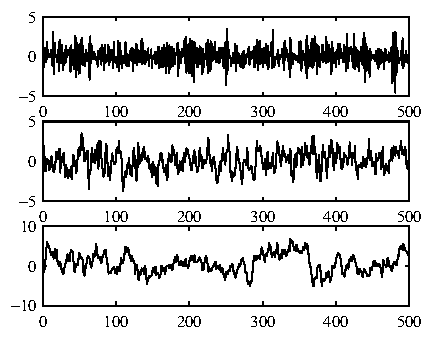
\includegraphics[width=0.6\textwidth]{Figures/chronoar1}\\
  \caption{Trajectoires de longueur $500$ d'un processus AR$(1)$ gaussien.
 Courbe du haut~: $\phi_1=-0.7$.
 Courbe du milieu~: $\phi_1=0.5$.
 Courbe du bas~: $\phi_1=0.9$}
 \label{fig:figar1}
\end{figure}

La fonction d'autocovariance de $(X_{t})$ solution stationnaire
de~(\ref{eq:recurrenceAR1}) est donn\'ee par la
formule~(\ref{eq:gamm_proc_lin}) qui s'\'ecrit\,;
\begin{align}
\label{eq:autocov:AR1}
\gamma_X(h)&= \sigma^2 \sum_{k=0}^\infty \phi_1^k \bar{\phi_1}\;^{k+h}
= \sigma^2 \frac{\bar{\phi_1}\;^{h}}{1 - |\phi_1|^2}\;,\;
\textrm{ si }h\geq 0\;,\\
&=\overline{\gamma(-h)}\;,\;\textrm{ sinon.}
\end{align}

Lorsque $\phi_1$ est un r\'eel strictement positif, le processus $(X_{t})$ est positivement
corr\'el\'e, dans le sens o\`u tous ses coefficients
d'auto-covariance sont positifs. Les exemples de trajectoires
repr\'esent\'ees sur la figure~\ref{fig:figar1} montrent que des valeurs
de $\phi_1$ proches de 1 correspondent \`a des trajectoires
``persistantes''. Inversement, des
valeurs de $\phi_1$ r\'eelles et n\'egatives conduisent \`a des trajectoires o\`u une valeur positive a tendance \`a \^{e}tre
suivie par une valeur n\'egative.
%====== FIGURE
\begin{figure}
\centering
  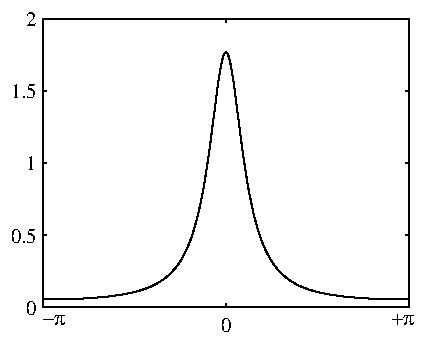
\includegraphics[width=0.6\textwidth]{Figures/dspthAR1}
  \caption{Densit\'e spectrale d'un processus AR(1), d\'efini
  par~(\ref{eq:recurrenceAR1}) pour $\sigma=1$ et $\phi_1=0.7$.}
  \label{fig:dspthAR1}
\end{figure}
la densit\'e spectrale de $(X_t)$ est donn\'ee par
\begin{equation}
\label{eq:dsp:AR1}
 f_X(\lambda)
 = \frac{\sigma^2}{2 \pi} \left| \sum_{k=0}^\infty \phi_1^k \rme^{-\rmi k\lambda} \right|^2
 = \frac{\sigma^2}{2 \pi} \frac{1}{|1 - \phi_1 \rme^{-\rmi \lambda}
   |^2}\; .
\end{equation}
%===============================================
\subsubsection{Cas $|\phi_1| > 1$}
%===============================================
Dans ce cas-l\`a, $\PE{|X_t-\sum_{j=0}^{k}\phi_1^j
Z_{t-j}|^2} = |\phi_1|^{2k+2} \PE{X_{t-k-1}^2}$ diverge
lorsque $k$ tend vers l'infini. Par contre, on peut
r\'e\'ecrire l'\'equation d\'efinissant $X_t$ en fonction de $Z_t$ comme suit
$$
X_t=-\phi_1^{-1} Z_{t+1}+\phi_1^{-1} X_{t+1}.
$$
En it\'erant l'\'equation pr\'ec\'edente, on obtient
\begin{eqnarray*}
X_t&=&-\phi_1^{-1} Z_{t+1}-\phi_1^{-2} Z_{t+2}+\phi_1^{-2} X_{t+2}=\dots\\
&=&-\phi_1^{-1} Z_{t+1}-\phi_1^{-2} Z_{t+2}-\dots-\phi_1^{-k-1}
Z_{t+k+1}+\phi_1^{-k-1} X_{t+k+1}\; .
\end{eqnarray*}
En utilisant exactement les m\^{e}mes arguments que ceux employ\'es
pr\'ec\'edemment, on d\'eduit que la solution stationnaire dans ce cas vaut
\begin{equation}
\label{eq:ar1_sol>1}
X_t=-\sum_{j\geq 1} \phi_1^{-j} Z_{t+j}\; .
\end{equation}
Cette solution est  \textbf{non causale} : elle d\'epend
uniquement du ``futur'' du processus $(Z_t)$.

Remarquons que, comme pr\'ec\'edemment, la solution donn\'ee par \eqref{eq:ar1_sol>1} est obtenu
en choisissant le d\'eveloppement fraction rationnelle $\psi(z)=(1-\phi_1
z^{-1})^{-1}$
\[
  \psi(z)=\frac{1}{1-\phi_1 z^{-1}} = \frac{-(\phi_1 z^{-1})^{-1}}{1-(\phi_1
    z^{-1})^{-1}}=-(\phi_1 z^{-1})^{-1}\sum_{k=0}^{+\infty} (\phi_1 z^{-1})^{-k}
=-\sum_{k\geq 1}\phi_1^{-k} z^{k}\;,
\]
qui converge sur le disque $ \ensemble{ z \in \Cset}{|z| < |\phi_1|}$. Nous remarquons que
nous avons choisi dans les deux cas $|\phi_1| < 1$ et $|\phi_1| > 1$ les d\'eveloppements convergeant
dans des domaines incluant le cercle unit\'e, $\ensemble{ z \in \Cset}{ |z|=1 }$.
Ce choix est justifié pr\'ecis\'ement dans le paragraphe \ref{sec:cas_general}.

%===============================================
\subsubsection{Cas $|\phi_1| = 1$}
%===============================================
Supposons qu'il existe une solution stationnaire dans ce cas alors,
par stationnarit\'e de $X_t$,
$$
\PE{\left|X_t - \sum_{j=0}^{k-1} \phi_1^j Z_{t-j}\right|^2} = |\phi_1|^{2k} \
\PE{|X_{t-k}|^2} = |\phi_1|^{2k}\ \PE{|X_{t}|^2}=\PE{|X_{t}|^2}\;.
$$
Or, le terme de gauche est aussi \'egal \`a
$$
\PE{|X_{t}|^2} + \PE{\left|\sum_{j=0}^{k-1} \phi_1^j Z_{t-j}\right|^2}
- 2 \PE{\bar{X}_{t} \sum_{j=0}^{k-1} \phi_1^j Z_{t-j}}\eqsp.
$$
Ainsi, $\PE{|\sum_{j=0}^{k-1} \phi_1^j Z_{t-j}|^2}
=2 \PE{\bar{X}_{t} \sum_{j=0}^{k-1} \phi_1^j Z_{t-j}}$.
De plus, $\PE{|\sum_{j=0}^{k-1} \phi_1^j Z_{t-j}|^2} = \sum_{j=0}^{k-1}
|\phi_1|^{2j} \sigma^2 = k \sigma^2 $. D'o\`u, en utilisant
l'in\'egalit\'e de Cauchy-Schwarz,
$$
k\sigma^2 \leq 2 \PE{|X_t|^2}^{1/2} \PE{\left|\sum_{j=0}^{k-1}
\phi_1^j Z_{t-j}\right|^2}^{1/2} \leq 2 (\gamma_X(0)+|\mu_X|^2)^{1/2} \
k^{1/2} \sigma \eqsp,
$$
ce qui est impossible pour $k$ grand.
Donc, dans ce cas, \textbf{il n'existe pas de solution stationnaire}.

\subsubsection{Conclusion}

Nous avons donc montr\'e, dans le cas $p=1$, que l'\'equation de  r\'ecurrence
(\ref{eq:recurrenceARp}) n'admettait pas de solution stationnaire
lorsque $|\phi_1|=1$ et qu'elle admettait une solution stationnaire
lorsque $|\phi_1|\neq 1$, donn\'ee par :
$$
X_t=\sum_{j\geq 0}\phi_1^j Z_{t-j}\;, \textrm{ si } |\phi_1|<1\;,
$$
et
$$
X_t=-\sum_{j\geq 1} \phi_1^{-j} Z_{t+j}\;, \textrm{ si } |\phi_1|>1\;.
$$

%
%\begin{definition}[Op\'erateur de retard]
%\label{def:operateur-retard}
%\index{Op\'erateur de retard}
%  Soit $(X_t)_{t\in\Zset}$ d\'efini sur $\espaceproba$ un processus stationnaire au
%  second ordre et soit $\cH^X_\infty$ son enveloppe lin\'eaire.
%D'apr\`es le th\'eor\`eme \ref{theo:prolongement-isometrie}, il existe une unique
%isom\'etrie $B^X$ de  $\cH^X_\infty$ dans $L^2\espaceproba$ telle que
%$B^X(X_t)=X_{t-1}$, pour tout $t\in\Zset$. De plus, $B^X(\cH^X_\infty)=\cH^X_\infty$.
% On appellera $B^X$ l'op\'erateur de retard de $X$ (abr\'eviation de {\em backward} en
%  anglais).
%\end{definition}
%
%On note $(B^X)^k = B^X \circ (B^X)^{k-1}$ pour $k \geq 1$ les compositions successives de
%l'op\'erateur $B^X$.  Pour $k<0$, $(B^X)^k$ est d\'efini comme l'op\'erateur inverse de
%$(B^X)^{-k}$. Cette notation permet d'\'ecrire les \'equations d\'efinissant un processus
%MA et un processus AR d'une fa\c{c}on plus condens\'ee : (\ref{eq:recurrenceMAq})
%se r\'e\'ecrit en : $X_t=\theta(B^Z)Z_t$ et (\ref{eq:recurrenceARp}) se r\'e\'ecrit
%en : $\phi(B^X)X_t=Z_t$ o\`u $\theta(z)=1+\sum_{k=1}^q \theta_k z^k$ et
%$\phi(z)=1-\sum_{k=1}^p \phi_k z^k.$
%%%%%%%%%%%%%%%%%%%%%%%%%%%%%%%%%%%%%%%%%%%%%%%%%%%%%%%%%%%%%%%%%%%%%%%%%%%%%%%%
%%%%%%%%%%%%%%%%%%%%%%%%%%%%%%%%%%%%%%%%%%%%%%%%%%%%%%%%%%%%%%%%%%%%%%%%%%%%%%%%


\subsection{Cas g\'en\'eral}\label{sec:cas_general}
% La notion de processus ARMA g\'en\'eralise les notions de processus MA
% et AR.
Avant d'\'enoncer le th\'eor\`eme \ref{theo:ARMApq} qui donne
une condition n\'ecessaire et suffisante d'existence d'une solution stationnaire
\`a l'\'equation r\'ecurrente \eqref{eq:recurrenceARMApq}
d\'efinissant un processus ARMA($p,q$), nous introduisons un nouvel op\'erateur
qui sera utile dans la preuve du th\'eor\`eme \ref{theo:ARMApq}.

Soit $\cS\espaceproba$ l'ensemble des processus index\'es par $\zset$
stationnaires au second ordre et \`a valeurs complexes. A toute suite de
coefficients complexes $(\alpha_k)$ v\'erifiant :
$\sum_{k\in\Zset}|\alpha_k|<\infty$, on associe un op\'erateur
$\operatorname{F}_\alpha$ qui \`a $X\in\cS\espaceproba$ associe le processus $Y$
d\'efini par :
$$
\operatorname{F}_\alpha:X\mapsto Y=(Y_t)_{t\in\Zset}=\left(\sum_{k\in\Zset}\alpha_k X_{t-k}\right)_{t\in\Zset}\; .
$$
D'apr\`es le th\'eor\`eme \ref{theo:filtragepassl_stat}, $Y$ est aussi dans $\cS\espaceproba$.

Le lemme \ref{lem:composition} montre comment composer deux op\'erateurs
de type $\operatorname{F}_\alpha$.

\begin{lemma}\label{lem:composition}
  Soient $(\alpha_k)$ et $(\beta_k)$ des suites de coefficients complexes
  telles que : $\sum_{k\in\Zset}|\alpha_k|<\infty$ et
  $\sum_{k\in\Zset}|\beta_k|<\infty$.  Si $X\in\cS\espaceproba$ alors
$$
\filtop{\alpha} \circ \filtop{\beta}X = \filtop{\alpha * \beta} X\;, \textrm{
  dans } L^2\espaceproba\;,\;
$$
o\`u $(\alpha*\beta)_k=\sum_{j\in\mathbb{Z}}\alpha_j\beta_{k-j}$ est la convolution discrète des suites $\alpha$ et $\beta$.
\end{lemma}

 \begin{proof}
 Soit $Y=\filtop{\beta}X$. D'apr\`es le th\'eor\`eme \ref{theo:filtragepassl_stat},
puisque $\sum_k|\beta_k|<\infty$, $Y$ est dans $\cS\espaceproba$.
Pour les m\^{e}mes raisons, $\filtop{\alpha}Y$ est lui aussi dans $\cS\espaceproba$.
Soient $Z=\filtop{\alpha}[\filtop{\beta}X]$ et $W=[\filtop{\alpha\beta}]X$, on a alors, pour tout $t\in\Zset$,
$Z_t=\sum_{j\in\Zset}\alpha_j Y_{t-j}$,
o\`u $Y_t=\sum_{k\in\Zset}\beta_k X_{t-k}$ et $W_t=\sum_{k\in\Zset}(\sum_{j\in\mathbb{Z}}\alpha_j\beta_{k-j})X_{t-k}$. Ainsi,
$Z_t=\sum_{j\in\Zset}\alpha_j(\sum_{k\in\Zset}\beta_k X_{t-j-k})$.

D\'efinissons $Z_{t,m,n}$ et $W_{t,m,n}$ par :
$Z_{t,m,n}=\sum_{j=-m}^m\alpha_j(\sum_{k=-n}^n\beta_k X_{t-j-k})$
et $W_{t,m,n}=\sum_{k=-m}^m(\sum_{j=-n}^n\alpha_j\beta_{k-j})X_{t-k}$.
En posant $\ell=j+k$, on en d\'eduit que
\begin{equation}\label{eq:chang_ind}
Z_{t,m,n}=\sum_{\ell=-(m+n)}^{m+n}(\sum_{j=-m}^m\alpha_j\beta_{\ell-j})X_{t-\ell}
=W_{t,m+n,m}\;.
\end{equation}
En notant $\| X \|_2 = \left( \PE{|X|^2} \right)^{1/2}$, nous pouvons
\'ecrire en utilisant l'in\'egalit\'e triangulaire que :
\begin{multline}\label{eq:dec_filtre1}
\|Z_t-W_t\|_2\leq \|Z_t-Z_{t,m,n}\|_2+\|Z_{t,m,n}-W_{t,m+n,m}\|_2
+\|W_{t,m+n,m}-W_t\|_2\;,
\end{multline}
le deuxi\`eme terme du membre de droite de (\ref{eq:dec_filtre1}) \'etant
nul d'apr\`es (\ref{eq:chang_ind}).
D'autre part, avec :
$Z_{t,m}=\sum_{j=-m}^m\alpha_j(\sum_{k\in\Zset}\beta_k X_{t-j-k})
=\sum_{j=-m}^m\alpha_j Y_{t-j}$, on a :
\begin{equation}\label{eq:dec_filtre2}
\|Z_t-Z_{t,m,n}\|_2\leq\|Z_t-Z_{t,m}\|_2+\|Z_{t,m}-Z_{t,m,n}\|_2\;.
\end{equation}
En utilisant l'in\'egalit\'e de Cauchy-Schwarz, le fait que
$Y$ est dans $\cS\espaceproba$ et $\sum_{k\in\Zset}|\alpha_k|<\infty$,  on a
\begin{multline}\label{eq:dec_filtre3}
\|Z_t-Z_{t,m}\|_2^2=\left\|\sum_{|j|>m}\alpha_j Y_{t-j}\right\|_2^2
\leq\PE{\sum_{|j|>m,|j'|>m}|\alpha_j| |\alpha_{j'}| |Y_{t-j}| |Y_{t-j'}|}\\
\leq \PE{Y_0^2}\left(\sum_{|j|>m} |\alpha_j|\right)^2\to 0\;,\; m\to\infty\;.
\end{multline}
D'autre part, en utilisant l'in\'egalit\'e de Cauchy-Schwarz, le fait que
$X$ est dans $\cS\espaceproba$ et l'absolue sommabilit\'e de $(\alpha_k)$
et $(\beta_k)$ :
\begin{align}\label{eq:dec_filtre4}
\|Z_{t,m}-Z_{t,m,n}\|_2^2&=\left\|\sum_{|j|\leq
  m}\alpha_j(\sum_{|k|>n}\beta_k X_{t-j-k})\right\|_2^2\\
&\leq \PE{X_0^2}\left(\sum_{-m\leq j,j'\leq m}|\alpha_j| |\alpha_{j'}|\right)
\left(\sum_{|k|,|k'|>n} |\beta_k||\beta_{k'}|\right)\\
&\leq \PE{X_0^2} \left(\sum_{j\in\Zset}|\alpha_j|\right)^2
\left(\sum_{|k|>n}|\beta_k|\right)^2\to 0\;,\; m,n\to\infty\;.
\end{align}
En utilisant (\ref{eq:dec_filtre2}), (\ref{eq:dec_filtre3}) et
(\ref{eq:dec_filtre4}), on obtient que le premier terme du membre de
droite de (\ref{eq:dec_filtre1}) tend vers 0 lorsque $m$ et $n$
tendent vers l'infini.
On peut montrer en utilisant le m\^{e}me type d'arguments que
$\|W_{t,m+n,m}-W_t\|_2$
tend vers 0 lorsque $m$ et $n$ tendent vers l'infini ce qui conclut la
preuve avec (\ref{eq:dec_filtre1}).

\end{proof}


\begin{theorem}[Existence et unicit\'e des processus ARMA$(p,q)$]
\label{theo:ARMApq} Soit l'\'equation r\'ecurrente~:
\begin{equation}
 \label{eq:recurrenceARMApq}
  X_t - \phi_1 X_{t-1} - \cdots - \phi_p X_{t-p}
  =
  Z_t + \theta_1 Z_{t-1} + \cdots + \theta_q Z_{t-q}\;,
\end{equation} o\`u $Z_t \sim \BB(0,\sigma^2)$ et les
$\phi_j$ et les $\theta_j$ sont des nombres complexes. On note $\phi(z)$ et $\theta(z)$ les transformées en $z$
\begin{align}
\label{eq:tz-phi}
\phi(z)&= 1 - \phi_1 z^{-1} - \dots - \phi_p z^{-p} \\
\label{eq:tz-theta}
\theta(z)&= 1 + \theta_1 z^{-1} + \dots + \theta_q z^{-q}  \eqsp.
\end{align}
On suppose que $\phi(z)$ et $\theta(z)$ n'ont pas de z\'eros communs. Alors l'\'equation
(\ref{eq:recurrenceARMApq}) admet une solution stationnaire au
second ordre si et seulement si le polyn\^ome $\phi(z) \neq 0$ pour
$|z| = 1$. Cette solution est unique et a pour expression~:
\begin{equation}
 \label{eq:solutionARMApq}
 X_t = \sum_{k=-\infty}^{\infty} \psi_k Z_{t-k}\;,
\end{equation}
o\`u les $(\psi_k)$ sont donn\'es par les coefficients du d\'eveloppement
\begin{equation}\label{eq:dev_laurent_statio}
\frac{\theta(z)}{\phi(z)}=\sum_{k\in\Zset}\psi_k z^{-k}\;,
\end{equation}
convergeant dans la couronne
\begin{equation}
\label{eq:RC-psi}
\ensemble{ z\in\cset}{\delta_1<|z|<\delta_2} \eqsp,
\end{equation}
o\`u $\delta_1<1$ et $\delta_2>1$ sont d\'efinis par
\begin{equation}
\label{eq:definition-delta1}
\delta_1=\max\{ z \in \cset, | z | < 1, \phi(z) =0 \}
\end{equation}
et
\begin{equation}
\label{eq:definition-delta2}
\delta_2=\min \{ z \in \cset, |z| > 1, \phi(z) = 0 \} \eqsp,
\end{equation}
\end{theorem}
avec la convention $\max \emptyset = 0$ et $\min \emptyset = \infty$.
\begin{proof}
Nous commen\c{c}ons par \'enoncer et prouver un lemme utile pour la preuve
du th\'eor\`eme \ref{theo:ARMApq}.
%\emnote{il faut se faire une religion ici sur la fa\c{c}on de noter les polynomes, pour le moment on est plut\^ot
%avec des petites lettres grecques, non.. ?}
\begin{lemma}\label{lem:dev_laurent}
  Soient $\theta$ et $\phi$ deux polyn\^omes \`a coefficients complexes tels que
  $\phi(z) \neq 0$ pour $|z|=1$ et $\phi(0)=1$ alors la fraction rationnelle
  $\theta(z)/\phi(z)$ est d\'eveloppable en s\'erie de Laurent, c'est-\`a-dire
$$
\frac{\theta(z)}{\phi(z)}=\sum_{k\in\Zset} c_k z^{-k}\;,
$$
o\`u la s\'erie $\sum_{k \in \zset} c_k z^{-k}$ est uniform\'ement convergente dans la
couronne d\'efinie par
$\left\{ z\in\cset \eqsp, r_1<|z|<r_2 \right\}$, o\`u
\begin{align*}
r_1&=\max\{ |z|~:~ z \in \cset, | z | < 1, \,\phi(z) =0 \}\\
r_2&=\min\{ |z|~:~ z  \in \cset, |z| > 1, \,\phi(z) = 0 \}\; .
\end{align*}
avec la convention $\max(\emptyset)=0$ et $\min(\emptyset)=\infty$.

Le cas $r_1=0$ correspond \`a $\phi(z)\neq0$ pour tout complexe $z$ tel que
$|z|\leq1$. Dans ce cas on a $c_k=0$ pour tout $k>0$.
Sinon, pour tout $\eta\in(0,r_1)$, $c_k=O(\eta^{-k})$ quand $k\to +\infty$.

Le cas $r_2=\infty$ correspond \`a $\phi(z)\neq0$ pour tout complexe $z$ tel que
$|z|\geq1$. Dans ce cas on a $c_k=0$ pour tout $k>\max(-1,\mathrm{deg}(\theta)
- \mathrm{deg}(\phi))$.  Sinon, pour tout $\eta\in(0,1/r_2)$, $c_k=O(\eta^{k})$
quand $k\to\infty$.
\end{lemma}
\begin{proof}\smartqed
  La d\'ecomposition en \'el\'ements simples de la fraction rationnelle
  $\theta(z)/\phi(z)$ s'\'ecrit comme la somme d'un polyn\^ome de degr\'e
  $\mathrm{deg}(\theta) - \mathrm{deg}(\phi)$ (avec la convention que tout
  polyn\^ome de degr\'e strictement n\'egatif est le polyn\^ome nul) et de termes de la forme~:
  $a/(z-z_0)^r$, o\`u $z_0$ est une racine de $\phi$ de multiplicit\'e sup\'erieure
  ou \'egale \`a $r$ et $a$ est une constante.  On \'ecrit :
\begin{align*}
\textrm{si }|z_0|<1,& \;
\frac{1}{(1-z_0 z^{-1})^r}=\frac{z^{-r}}{(1-z_0/z)^r},\;
\textrm{lorsque }|z_0|<|z|\;,\\
\textrm{si }|z_0|>1,& \;
\frac{1}{(z-z_0)^r}=\frac{(-z_0)^{-r}}{(1-z/z_0)^r},\;
\textrm{lorsque }|z|<|z_0|\;.
\end{align*}
%\emnote{ce n'est que le DL de $(1-u)^\alpha$ on n'a pas besoin de trop disserter dessus}
On utilise que :
\begin{multline*}
(1-u)^{-r}=\frac{(-1)^{r-1}}{(r-1)!}\sum_{k\geq r-1}\frac{k!}{(k-r+1)!}
u^{k-r+1}\\
=\frac{(-1)^{r-1}}{(r-1)!}\sum_{k\geq 0}\frac{(k+r-1)!}{k!}
u^{k}\;,\textrm{ lorsque }|u|<1\;,
\end{multline*}
Ainsi,
\begin{align*}
&\textrm{si }|z_0|<1, \;
\frac{1}{(z-z_0)^r}=\frac{z^{-r}}{(1-z_0/z)^r}
=z^{-r}\frac{(-1)^{r-1}}{(r-1)!}\sum_{k\geq 0}\frac{(k+r-1)!}{k!}(z_0/z)^k,\; \\
&\textrm{qui converge si }|z_0|<|z|\;,\\
&\textrm{si }|z_0|>1, \;
\frac{1}{(z-z_0)^r}=\frac{(-z_0)^{-r}}{(1-z/z_0)^r}
=-\frac{z_0^{-r}}{(r-1)!}\sum_{k\geq 0}\frac{(k+r-1)!}{k!}
(z/z_0)^k,\; \\
&\textrm{qui converge si }|z|<|z_0|\;.
\end{align*}
En majorant $(k+r-1)!/k!$ par $k^{r-1}$, on en d\'eduit  que
\begin{align*}
&\textrm{si }|z_0|<1, \;
\frac{1}{(z-z_0)^r}=\sum_{k\leq -r} v_k z^k,\; \textrm{qui converge si }|z|>|z_0|\;,\\
&\textrm{si }|z_0|>1, \;
\frac{1}{(z-z_0)^r}=\sum_{k\geq 0} w_k z^k,\;\textrm{qui converge si }|z|<|z_0|\;,
\end{align*}
o\`u $|v_k|$ et $|w_k|$ sont major\'es par $C \eta^{|k|}$, $C$ \'etant une constante
strictement positive pour tout $\eta$ choisi dans
$(0,r_1)$ ou $(0,1/r_2)$, respectivement.

\end{proof}

\textbf{Retour \`a la preuve du th\'eor\`eme \ref{theo:ARMApq}}\\

Supposons que $\phi(z)\neq 0$ pour $|z|= 1$, alors d'apr\`es
le \Cref{lem:dev_laurent} il existe $r_1<1$ et $r_2>1$ tels que
\begin{equation}\label{eq:psi_arma}
\psi(z)=\frac{\theta(z)}{\phi(z)}=\sum_{k=-\infty}^{\infty} \psi_k z^{-k},\; r_1<|z|<r_2\;,
\end{equation}
o\`u la suite $(\psi_k)_{k\in\Zset}$ v\'erifie $\sum_k |\psi_k|<\infty$.
V\'erifions que le processus $(X_t)$ d\'efini par : $X_t=\sum_{k\in\Zset} \psi_k Z_{t-k}=(\filtop{\psi} Z)_t$, pour tout
$t\in\Zset$ est une solution stationnaire de (\ref{eq:recurrenceARMApq}). D'apr\`es la d\'efinition
\ref{def:proc_lin}, $(X_t)$ est stationnaire. De plus, d'apr\`es le \Cref{lem:composition},
$$
\filtop{\phi} \circ \filtop{\psi} Z =\filtop{\phi*\psi}Z=\filtop{\theta}Z \eqsp,
$$
ce qui montre l'existence d'une solution
stationnaire \`a \eqref{eq:recurrenceARMApq}.

D'autre part, si $X$ est un processus stationnaire au second ordre solution de
(\ref{eq:recurrenceARMApq}) alors $X$ v\'erifie :
\begin{equation}\label{eq:arma_F}
\filtop{\phi} X=\filtop{\theta}Z\;.
\end{equation}
Comme $\phi(z)\neq 0$ pour $|z|= 1$, alors d'apr\`es le
\Cref{lem:dev_laurent} il existe $r_1<1$ et $r_2>1$ tels que :
$$
\xi(z)=\frac{1}{\phi(z)}=\sum_{k\in\Zset} \xi_k z^{k},\; r_1<|z|<r_2\;,
$$
o\`u la suite $(\xi_k)_{k\in\Zset}$ v\'erifie $\sum_k |\xi_k|<\infty$.
On peut donc appliquer l'op\'erateur $\filtop{\xi}$ aux deux membres de l'\'equation
(\ref{eq:arma_F}) d'o\`u l'on d\'eduit en utilisant le lemme \ref{lem:composition}
que $X=\filtop{\xi\theta}Z=\filtop\psi Z$ o\`u $(\psi_k)$ est d\'efinie dans (\ref{eq:psi_arma}).
Donc $X_t=\sum_{k\in\Zset} \psi_k Z_{t-k}=(\filtop{\psi} Z)_t$, pour tout
$t\in\Zset$, ce qui assure l'unicit\'e de la solution.

R\'eciproquement, si $(X_t)$ est un processus stationnaire solution de (\ref{eq:recurrenceARMApq}) de la forme
$X_t=\sum_{k\in\Zset}\eta_k Z_{t-k}$ o\`u $\sum_k |\eta_k|<\infty$, montrons que
$\phi(z)\neq 0$ pour $|z|= 1$. En effet, puisque $X$ est solution de (\ref{eq:arma_F})
alors : $\filtop{\phi} X=\filtop{\phi}[\filtop{\eta} Z]=\filtop{\theta} Z$. D'apr\`es le lemme \ref{lem:composition},
$\filtop{\phi\eta}Z=\filtop{\theta} Z$. Posons
$\zeta_k=\sum_{j\in\Zset}\phi_j \eta_{k-j}$. On a alors, pour tout $t\in\Zset$,
$\sum_{k\in\Zset}\zeta_k Z_{t-k}=\sum_{j=1}^q\theta_j Z_{t-j}.$
En multipliant les deux membres de cette \'equation par $Z_{t-\ell}$
et en prenant l'esp\'erance, on d\'eduit que $\zeta_\ell=\theta_\ell$,
$\ell=0,\dots,q$ et $\zeta_\ell=0$, sinon. Ainsi,
$\theta(z)=\phi(z)\eta(z)$, $|z|=1$. Puisque $\theta$ et $\phi$
n'ont pas de racines communes et que $|\eta(z)|\leq\sum_{k\in\Zset}|\eta_k|<\infty$,
si $|z|=1$, $\phi(z)$ ne s'annule pas sur le cercle unit\'e :
$\{z,\; |z|=1\}$, ce qui conclut la preuve du th\'eor\`eme \ref{theo:ARMApq}.

% Supposons que $\phi(z)\neq 0$ pour $|z|= 1$, alors d'apr\`es le lemme
% \ref{lem:dev_laurent} il existe $r_1<1$ et $r_2>1$ tels que
% $$
% \psi(z)=\frac{\theta(z)}{\phi(z)}=\sum_{k=-\infty}^{\infty} \psi_k z^{k},\; r_1<|z|<r_2\;,
% $$
% o\`u la suite $(\psi_k)_{k\in\Zset}$ v\'erifie $\sum_k |\psi_k|<\infty$.
% V\'erifions que $X_t=\sum_{k\in\Zset} \psi_k Z_{t-k}=\psi(B^Z)Z_t$ pour tout
% $t\in\Zset$ est une solution stationnaire de (\ref{eq:recurrenceARMApq}). D'apr\`es la d\'efinition
% \ref{def:proc_lin}, $(X_t)$ est stationnaire. De plus, par d\'efinition, $\cH^X_\infty\subset\cH^Z_\infty$ et
% d'apr\`es le lemme \ref{lem:composition},
% $\phi(B^Z)X_t=\phi(B^Z)\psi(B^Z)Z_t=(\phi\psi)(B^Z)Z_t=\theta(B^Z)Z_t.$
% Montrons que cette solution est unique. Pour cela, notons En effet, soit $(Y_t)$ un autre processus stationnaire
% solution de (\ref{eq:recurrenceARMApq}) alors :
% $(X_t-Y_t)-\sum_{k=1}^p\phi_k(X_{t-k}-Y_{t-k})=0$


% R\'eciproquement, si $X_t$ est une solution stationnaire de (\ref{eq:recurrenceARMApq}) de la forme
% $X_t=\sum_{k\in\Zset}\eta_k Z_{t-k}$ o\`u $\sum_k |\eta_k|<\infty$
% alors : $\phi(B^X)X_t=\phi(B^Z)\eta(B^Z)Z_t=\theta(B^Z)Z_t$. D'apr\`es le lemme \ref{lem:composition},
% $(\phi\eta)(B^Z)Z_t=\theta(B^Z)Z_t$. Posons
% $\zeta(z)=\phi(z)\eta(z)=\sum_{k\in\Zset}\zeta_k z^k$, lorsque $|z|=1$. On a alors,
% $\sum_{k\in\Zset}\zeta_k Z_{t-k}=\sum_{j=1}^q\theta_j Z_{t-j}.$
% En multipliant les deux membres de cette \'equation par $Z_{t-\ell}$
% et en prenant l'esp\'erance, on d\'eduit que $\zeta_\ell=\theta_\ell$,
% $\ell=0,\dots,q$ et $\zeta_\ell=0$, sinon. Ainsi,
% $\theta(z)=\phi(z)\eta(z)$, $|z|=1$. Puisque $\theta$ et $\phi$
% n'ont pas de racines communes et que $|\eta(z)|\leq\sum_{k\in\Zset}|\eta_k|<\infty$,
% si $|z|=1$, $\phi(z)$ ne s'annule pas sur le cercle unit\'e :
% $\{z,\; |z|=1\}.$

\end{proof}
Dans le cas o\`u $\phi(z)$ et $\theta(z)$ ont des z\'eros communs,
deux configurations sont possibles~:
\begin{enumerate}[label=(\alph*)]
\item Les z\'eros communs ne sont pas sur le cercle unit\'e. Dans ce
cas on se
  ram\`ene au cas sans z\'ero commun en annulant les facteurs communs.
\item Certains des z\'eros communs se trouvent sur le cercle unit\'e.
  L'\'equation~(\ref{eq:recurrenceARMApq}) admet une infinit\'e de solutions
  stationnaires au second ordre.
\end{enumerate}
Du point de vue de la mod\'elisation, la pr\'esence de z\'eros communs
ne pr\'esente aucun int\'er\^{e}t puisqu'elle est sans influence sur
la densit\'e spectrale de puissance. Elle conduit de plus \`a une
ambigu\"{i}t\'e sur l'ordre r\'eel des parties AR et MA.
%=========================================================
\subsubsection{ARMA$(p,q)$ causal}
%  Comme dans le cas d'un processus AR($p$), on peut
% distinguer trois cas, suivant que les z\'eros de $\phi(z)$ sont \`a
% l'ext\'erieur, \`a l'int\'erieur ou de part et d'autre du cercle unit\'e.
% Dans le cas o\`u les z\'eros de $\phi(z)$ sont \`a l'ext\'erieur du
% cercle unit\'e, la suite $\xi_k$ est causale ($\xi_k=0$ pour $k<0$)
% et donc $\psi_k=\xi_k+\sum_{j=1}^q \theta_j\xi_{k-j}$ est aussi
% causale. Par cons\'equent le processus $X_t$ s'exprime causalement
% en fonction de $Z_t$.
Le th\'eor\`eme \ref{theo:ARMApq_causal} donne une condition n\'ecessaire
et suffisante d'existence d'une solution causale \`a l'\'equation
(\ref{eq:recurrenceARMApq}).

\begin{definition}[Repr\'esentation ARMA causale]
  Sous les hypoth\`eses du th\'eor\`eme~\ref{theo:ARMApq}, on dira que
  l'\'equation~(\ref{eq:recurrenceARMApq}) fournit une repr\'esentation causale de
  la solution stationnaire au second ordre $(X_t)$ si $(X_t)_{t\in\zset}$ est
  un processus lin\'eaire causal par rapport \`a $(Z_t)_{t\in\zset}$.
\end{definition}

\begin{theorem}[ARMA$(p,q)$ causal]
\label{theo:ARMApq_causal}
Soit l'\'equation r\'ecurrente~:
\begin{equation}
 \label{eq:recurrenceARMApqcausal}
  X_t - \phi_1 X_{t-1} - \cdots - \phi_p X_{t-p}
  =
  Z_t + \theta_1 Z_{t-1} + \cdots + \theta_q Z_{t-q}
\end{equation} o\`u $Z_t \sim \BB(0,\sigma^2)$ et
$\{ \phi_j \}_{j = 1}^p$ et $\{ \theta_j \}_{j=1}^q$ sont des nombres complexes. On pose
$\phi(z)= 1 - \phi_1 z^{-1} - \dots - \phi_p z^{-p}$ et $\theta(z)= 1 +
\theta_1 z^{-1} + \dots + \theta_p z^{-p}$. On suppose que $\phi(z)$ et
$\theta(z)$ n'ont pas de z\'eros communs. Alors l'\'equation
(\ref{eq:recurrenceARMApqcausal})
fournit une repr\'esentation causale de la solution stationnaire au second ordre
si et seulement si le polyn\^ome $\phi(z)
\neq 0$ pour $|z| \geq 1$. Cette solution a pour
expression~:
\begin{equation}
 \label{eq:solutionARMApq_causal}
  X_t = \sum_{k\geq 0} \psi_k Z_{t-k}
\end{equation}
o\`u la suite $(\psi_k)$ est donn\'ee par les coefficients du d\'eveloppement
$$
\frac{\theta(z)}{\phi(z)}=\sum_{k=0}^{\infty} \psi_k z^{-k}
$$
qui converge dans la couronne $\{z\in\cset\;,\;|z|\geq 1\}.$
\end{theorem}
\begin{proof}\smartqed
Le th\'eor\`eme~\ref{theo:ARMApq} montre l'existence et l'unicit\'e
de la solution de l'\'equation~(\ref{eq:recurrenceARMApqcausal}) et v\'erifie
\begin{equation*}
  X_t = \sum_{k\in\zset} \psi_k Z_{t-k}
\end{equation*}
o\`u la suite $(\psi_k)$ est caract\'eris\'ee par l'\'equation
$$
\frac{\theta(z)}{\phi(z)}=\sum_{k=0}^{\infty} \psi_k z^{-k},\quad z\in\cset,\,|z|=1\;.
$$
Si maintenant $\phi(z)\neq 0$ pour $|z|\leq 1$, alors, d'apr\`es le
 lemme \ref{lem:dev_laurent}, comme $r_1=0$, on a $\psi_k=0$ pour $k<0$
 et~(\ref{eq:solutionARMApq_causal}) suit.


R\'eciproquement, si $X$ est une solution stationnaire de
(\ref{eq:recurrenceARMApqcausal}) de la forme $X_t=\sum_{k\geq 0}\eta_k
Z_{t-k}$ o\`u $\sum_k |\eta_k|<\infty$, montrons que $\phi(z)\neq 0$ pour
$|z|\leq 1$. En effet, puisque $X$ est solution
de~(\ref{eq:recurrenceARMApqcausal}), alors : $\filtop{\phi}
X=\filtop{\phi}[\filtop{\eta} Z]=\filtop{\theta} Z$. D'apr\`es le lemme
\ref{lem:composition}, $\filtop{\phi\eta}Z=\filtop{\theta} Z$. Posons, pour
tout $k\in\mathbb{N}$, $\zeta_k=\sum_{j\geq 0}\phi_j \eta_{k-j}$, o\`u par
convention, $\eta_\ell=0$, si $\ell<0$.  On a alors, pour tout $t\in\Zset$,
$\sum_{k\geq 0}\zeta_k Z_{t-k}=\sum_{j=0}^q\theta_j Z_{t-j},$ avec la
convention $\theta_0=1$.  En multipliant les deux membres de cette \'equation par
$Z_{t-\ell}$ et en prenant l'esp\'erance, on d\'eduit que $\zeta_\ell=\theta_\ell$,
$\ell=0,\dots,q$ et $\zeta_\ell=0$, sinon. Ainsi, $\theta(z)=\phi(z)\eta(z)$,
$|z|\leq 1$. Puisque $\theta$ et $\phi$ n'ont pas de racines communes et que
$|\eta(z)|\leq\sum_{k\geq 0}|\eta_k|<\infty$, si $|z|\leq 1$, $\phi(z)$ ne
s'annule pas sur le disque unit\'e : $\{z,\; |z|\leq 1\}$, ce qui conclut la
preuve du th\'eor\`eme~\ref{theo:ARMApq_causal}.

\end{proof}
%==========================================


\begin{definition}[Repr\'esentation ARMA inversible]
  Sous les hypoth\`eses du th\'eor\`eme~\ref{theo:ARMApq}, on dira que
  l'\'equation~(\ref{eq:recurrenceARMApq}) fournit une repr\'esentation inversible
  de la solution stationnaire au second ordre $(X_t)$ si $(X_t)_{t\in\zset}$
  est un processus lin\'eaire inversible par rapport \`a $(Z_t)_{t\in\zset}$.
\end{definition}

\begin{theorem}[ARMA$(p,q)$ inversible]
 \label{theo:ARMAinversible}
Soit l'\'equation r\'ecurrente~:
\begin{equation}
 \label{eq:recurrenceARMApqinversible}
  X_t - \phi_1 X_{t-1} - \cdots - \phi_p X_{t-p}
  =
  Z_t + \theta_1 Z_{t-1} + \cdots + \theta_q Z_{t-q}
\end{equation} o\`u $Z_t \sim \BB(0,\sigma^2)$ et les
$\phi_j$ et les $\theta_j$ sont des nombres complexes. On pose
$\phi(z)= 1 - \phi_1 z - \dots - \phi_p z^p$ et $\theta(z)= 1 +
\theta_1 z + \dots + \theta_p z^p$. On suppose que $\phi(z)$ et
$\theta(z)$ n'ont pas de z\'eros communs. Alors l'\'equation
(\ref{eq:recurrenceARMApqinversible}) fournit une repr\'esentation inversible
de la solution stationnaire au second ordre si et seulement si le polyn\^ome $\theta(z)
\neq 0$ pour $|z| \leq 1$. Cette solution est unique et a pour
expression~:
\begin{equation}
 \label{eq:solutionARMApq_inversible}
  Z_t = \sum_{k\geq 0} \pi_k X_{t-k}
\end{equation}
o\`u la suite $(\pi_k)$ est donn\'ee par les coefficients du d\'eveloppement
$$
\frac{\phi(z)}{\theta(z)}=\sum_{k=0}^{\infty} \pi_k z^{-k}
$$
qui converge dans $\{z\in\cset\;,\;|z|\leq 1\}.$
% Soit $X_t$ un processus ARMA$(p,q)$. On suppose que $\phi(z)$ et
% $\theta(z)$ n'ont pas de z\'eros communs. Alors il existe une suite
% $\{\pi_k\}$ causale absolument sommable telle que~:
% \begin{equation}
%  \label{eq:analyseARMApq}
%  Z_t=\sum_{k=0}^{\infty} \pi_k X_{t-k}
% \end{equation}
% si et seulement si $\theta(z)\neq 0$ pour $z\leq 1$. On dit alors
% que le mod\`ele ARMA$(p,q)$ est inversible. La suite $\pi_k$ est
% la suite des coefficients du d\'eveloppement en s\'erie de
% $\phi(z)/\theta(z)$ dans le disque $\{z: |z|\leq 1\}$.
\end{theorem}
La preuve de ce th\'eor\`eme est tout \`a fait analogue \`a celle du
th\'eor\`eme~\ref{theo:ARMApq_causal} et n'est donc pas d\'etaill\'ee ici.
% Remarquons que la notion d'inversibilit\'e, comme celle de causalit\'e, est bien relative au
% mod\`ele ARMA$(p,q)$ lui-m\^{e}me et pas uniquement au processus
% $X_t$.
%\begin{exercice}
%  Soit $X_t$ un processus stationnaire au second ordre solution de l'\'equation
%  de r\'ecurrence~(\ref{eq:recurrenceARMApqcausal}) o\`u le mod\`ele ARMA$(p,q)$
%  correspondant est suppos\'e sans z\'ero commun mais pas n\'ecessairement
%  inversible. Montrer qu'il existe un bruit blanc $\tilde{Z}_t$ tel que $X_t$
%  soit solution de
%  \[
%    \phi(B) X_t = \tilde{\theta}(B) \tilde{Z}_t
%  \]
%  o\`u le mod\`ele ARMA$(p,q)$ d\'efini par $\phi_1, \dots \phi_p$ et
%  $\tilde{\theta}_1, \dots \tilde{\theta}_q$ est inversible
%  (indication\,: consid\'erer des facteurs passe-tout).
%\end{exercice}

Un mod\`ele ARMA$(p,q)$ est causal et inversible lorsque
les racines des polyn\^omes $\phi(z)$ et $\theta(z)$ sont toutes
situ\'ees \`a l'ext\'erieur du disque unit\'e. Dans ce cas, $X_t$ et $Z_t$
se d\'eduisent mutuellement l'un de l'autre par des op\'erations de
filtrage causal.
%, la r\'eponse impulsionnelle de chacun de ces
%filtres \'etant {\em \`a phase minimale} (c'est \`a dire inversible
%causalement).

\subsubsection{Calcul des covariances d'un processus ARMA$(p,q)$ causal}
Une premi\`ere m\'ethode consiste \`a utiliser l'expression
(\ref{eq:gamm_proc_lin}) % qui s'\'ecrit, compte tenu du fait que
% $\{Z_t\}$ est un bruit blanc,
% $$
%  \gamma(h)=
%    \sigma^2 \sum_{k=0}^\infty\psi_k \psi_{k+|h|}
%    $$
   o\`u la suite $(\psi_k)$ se d\'etermine de fa\c{c}on r\'ecurrente \`a partir de
   l'\'egalit\'e $\psi(z)\theta(z)=\phi(z)$ par identification du terme en $z^k$.
   Pour les premiers termes on trouve~:
\begin{eqnarray*}
 &&\psi_0=1\\
 &&\psi_1=\theta_1+\psi_0\phi_1\\
 &&\psi_2=\theta_2+\psi_0\phi_2+\psi_1\phi_1\\
 &&\cdots
\end{eqnarray*}
La seconde m\'ethode utilise une formule de r\'ecurrence, v\'erifi\'ee par
la fonction d'autocovariance d'un processus ARMA$(p,q)$, qui
s'obtient en multipliant les deux membres de
(\ref{eq:recurrenceARMApq}) par $\bar{X}_{t-k}$ et en prenant
l'esp\'erance. On obtient~:
\begin{align}
 \label{eq:recurrencegamma1}
  &\gamma(k)-\phi_1\gamma(k-1)-\cdots-\phi_p\gamma(k-p)
  =
  \sigma^2\sum_{k\leq j\leq q}\theta_j\bar{\psi}_{j-k}\;,\;
0\leq k < \max(p,q+1)
  \\
 \label{eq:recurrencegamma2}
  &\gamma(k)-\phi_1\gamma(k-1)-\cdots-\phi_p\gamma(k-p)
  =
  0\;,\; k \geq \max(p,q+1)
\end{align}
o\`u nous avons utilis\'e la causalit\'e du processus pour \'ecrire
que $\PE{Z_t \bar{X}_{t-k}}=0$ pour tout $k\geq 1$. Le calcul de la
suite $\{\psi_k\}$ pour $k=1,\dots, p$ se fait comme pr\'ec\'edemment.
En reportant ces valeurs dans~(\ref{eq:recurrencegamma1}) pour
$0\leq k \leq p$, on obtient $(p+1)$ \'equations lin\'eaires aux
$(p+1)$ inconnues $(\gamma(0),\dots,\gamma(p))$ que l'on peut
r\'esoudre. Pour d\'eterminer les valeurs suivantes on utilise
l'expression (\ref{eq:recurrencegamma2}).
\subsubsection{Densit\'e spectrale d'un processus ARMA$(p,q)$}
\begin{theorem}[Densit\'e spectrale d'un processus ARMA$(p,q)$]
Soit $(X_t)$ un processus ARMA$(p,q)$ (pas n\'ecessairement causal ou
inversible) \textit{i.e.} la solution stationnaire de l'\'equation
(\ref{eq:recurrenceARMApq}) o\`u les polyn\^omes $\theta(z)$ et $\phi(z)$ sont des
polyn\^omes de degr\'e $q$ et $p$ n'ayant pas de z\'eros communs. Alors
$(X_t)$ poss\`ede une densit\'e spectrale qui a pour expression~:
\begin{equation}
 \label{eq:dspARMApq}
 f(\lambda)=\frac{\sigma^2}{2\pi}
    \frac{\left| 1+\sum_{k=1}^q \theta_k \rme^{-\rmi k \lambda}\right|^2}
         {\left| 1-\sum_{k=1}^p \phi_k \rme^{-\rmi k \lambda}\right|^2}\;,\; -\pi\leq\lambda\leq\pi\;.
\end{equation}
\end{theorem}

\begin{remark}
D'apr\`es le th\'eor\`eme \ref{theo:ARMApq}, l'expression de $f$ est bien
d\'efinie puisque $\phi$ ne s'annule pas sur le cercle unit\'e.
\end{remark}





%%% Local Variables:
%%% mode: latex
%%% ispell-local-dictionary: "francais"
%%% TeX-master: "../monographie-serietemporelle"
%%% End:
